\documentclass{article}
\usepackage[utf8]{inputenc}
\usepackage{array}
\usepackage{wrapfig}
\usepackage{multirow}
\usepackage{tabu}
\usepackage{graphicx}
\usepackage{float} 
\title{CENG 499 HW1 Report}
\author{Ahmet Berker KOÇ \\ 2232320}
\date{25.04.2021}

\begin{document}
\maketitle

\section{Sanity Checks}
Since we know that our dataset is balanced, we can do the following checks.

\subsection{Loss}
We use cross entropy loss and we know that the dataset is balanced. Therefore, every class has equal probability and there are 10 (N) classes. After random initialization, I print the loss and I saw -2.30 loss \\
The calculation as follows \\ \\ 
$-\log \frac{1}{N} $ \\ \\
In our case N=10\\ \\ 
$-\log \frac{1}{10} = 2.30258509299  $ \\



\subsection{Accuracy}
The dataset is balanced. Therefore; I expected that accuracy is equal to randomness (probabilty of N class). Accuracy should be around $\frac{1}{N}$. In our case, class is equal to 10. So accuracy is $\frac{1}{10}$ after random initialization. I also print it and I saw the accuracy as 10.01 percent or 9.98 percent.  

\section{Separating Validation Set}
While I was spliting training and validation sets, I benefited from pytorch torch.utils.data.randomsplit function. I obtained 25000 image for training and 5000 image for validation. This seperation is done randomly thanks to the pytorch function. 

\section{Hyperparameter optimization}

\subsection{1-layer (0-hidden-layer) network}

In this part I use 1 layer network. I train 6 models for different learning rate(hyperparameter). It gave accuracy around 0.3  as expected. This accuracy values are obtained by using validation part of the code and validation set.  The least accuracy 21.16 is obtained in biggest learning rate 0.03. 

Not: I write accuracy value in the table. I also put the loss and share at the end of the document. The accuracy values are percent values for more comfotable reading.\\

My some learning rates are different from the document given. \\

My learning rates are   0.01, 0.03, 0.001, 0.003, 0.0001, 0.0003 \\



\begin{table}[htbp]
    \centering
    \begin{tabular}{|c|c|c|c|c|c|c|}
    \hline
    \multirow{2}{5em}{AF and HS} & \multicolumn{6}{c|}{Learning Rate} \\
        & 0.01 & 0.03 & 0.001 & 0.003 & 0.0001 & 0.0003 \\
        \hline \hline
        -, -  & 32.32 & 21.16 & 38.30 & 35.00 & 38.96 & 38.62 \\
        \hline
    \end{tabular}
    \caption{1-layer network}
    \label{tab:1layer}
\end{table}


\newpage
\subsection{2-layer (1-hidden-layer) network}

In this part I use 2 layer network. I train 6 models for different learning rate(hyper-parameter), 3 different neuron, and 3 different activation function. I totally made 54 experiment and obtained 54 different model. Some model diverges because of the learning rate. Especially,models which have 0.01, 0.03 and 0.003 learning rates tend to diverge. On the other hand, models with 0.001, 0.0001 and 0.0003 learning rates tend to converge. Models which diverge gave the accuracy around 0.10 which is equal to probability of 10 class. Models which converge gave the good accuracy between 45-55. This results are also expected.\\
Note:\\
Activation functions are S:sigmoid, T:tanh, R:ReLU.\\
Number of Neuron are 256, 512, 1024 \\


\begin{table}[htbp]
    \centering
    \begin{tabular}{|c|c|c|c|c|c|c|c|c|}
    \hline
    \multirow{2}{5em}{Layer Activations} & \multicolumn{6}{c|}{Learning Rate} \\
        & 0.01 & 0.03 & 0.001 & 0.003 & 0.0001 & 0.0003 \\
        \hline \hline
        S, 256  & 11.02 & 9.63 & 47.82 & 10.24 & 44.62 & 55.00 \\
        S, 512  & 9.72 & 9.44 & 48.54 & 11.02 & 46.30 & 55.46 \\
        S, 1024  & 9.92 & 9.64 & 49.04 & 9.92 & 47.64 & 55.38 \\
        T, 256  & 9.96 & 11.02 & 19.26 & 9.92 & 50.68 & 55.06 \\
        T, 512  & 10.26 & 9.72 & 31.04 & 9.44 & 52.54 & 55.28 \\
        T, 1024  & 10.12 & 9.63 & 9.92 & 10.26 & 52.58 & 56.20 \\
        R, 256  & 10.12 & 11.02 & 51.56 & 21.50 & 44.80 & 53.80 \\
        R, 512  & 10.12 & 11.02 & 52.81 & 21.28 & 53.22 & 53.84 \\
        R, 1024  & 10.12 & 11.02 & 55.66 & 10.24 & 52.92 & 56.66 \\
        \hline
    \end{tabular}
    \caption{2-layer network}
    \label{tab:2layer}
\end{table}


\newpage
\subsection{3-layer (2-hidden-layer) network}

In this part I use 3 layer network. I train 6 models for different learning rate(hyper-parameter), 3 different neuron, and 3 different activation function. I totally made 54 experiment and obtained 54 different model. Some model diverges because of the learning rate. Especially, 0.01, 0.03 and 0.003 learning rates tend to diverge. Compared to 2 layer, some models(R,512 and R,1024)which have 0.003 and 0.01 doesn't diverge.  Models with 0.001, 0.0001 and 0.0003 learning rates tend to converge similarly. Models which diverge gave the accuracy around 0.10 which is equal to probability of 10 class. Models which converge gave the good accuracy around 50-55. This results are also expected. \\

The highest accuracy of all models is 58.46


\begin{itemize}
	\item Learning Rate = 0.0001 
	\item Neuron = 512
	\item Activation Function = tanh
	\item Layer = 3 layer (2 hidden layer)
\end{itemize}

Note:\\
Activation functions are S:sigmoid, T:tanh, R:ReLU.\\
Number of Neuron are 256, 512, 1024 \\

\begin{table}[htbp]
    \centering
    \begin{tabular}{|c|c|c|c|c|c|c|c|c|}
    \hline
    \multirow{2}{5em}{Layer Activations} & \multicolumn{6}{c|}{Learning Rate} \\
        & 0.01 & 0.03 & 0.001 & 0.003 & 0.0001 & 0.0003 \\
        \hline \hline
        S, 256  & 9.72 & 10.24 & 48.08 & 10.26 & 54.30 & 55.28 \\
        S, 512  & 10.12 & 11.02 & 38.18 & 10.26 & 54.70 & 55.02  \\
        S, 1024  & 11.02 & 10.12 & 30.08 & 10.24 & 54.94 & 53.68 \\
        T, 256  & 10.26 & 10.26 & 9.64 & 9.64 & 57.06 & 55.58 \\
        T, 512  & 9.64 & 9.68 & 9.68 & 9.64 & 58.46 & 54.50\\
        T, 1024  & 10.24 & 10.24 & 9.72 & 9.96 & 57.28 & 54.58 \\
        R, 256  & 20.80 & 10.26 & 57.80 & 10.12 & 56.22 & 56.94 \\
        R, 512  & 11.02 & 10.12 & 58.35 & 40.50 & 56.92 & 57.54 \\
        R, 1024  & 30.04 & 9.68 & 57.62 & 32.18 & 56.70 & 57.94 \\
        \hline
    \end{tabular}
    \caption{3-layer network}
    \label{tab:3layer}
\end{table}

\section{The best hyperparameter}
\subsection{Results}
Hyper parameter settin of my network which give the best validation result and I tested it
\begin{itemize}
	\item Learning Rate = 0.0001 
	\item Neuron = 512
	\item Activation Function = tanh
	\item Layer = 3 layer (2 hidden layer)
\end{itemize}

I run my test code and obtained the labels for test data set. Then, I put the file with image name and predicted labels of them. I gave the accuracy as 0.572900 \\

In Figure 1, there is my training and validation curve for 60 epoch. I stop the code in 40th epoch. My last model save is 36th epoch. It is the minimum validation loss point. As seen in the Figure 1, After 36-40'th epoch, validation loss is increase even if training loss continue to decrease. This means that model overfit. Therefore, I save the model according to minimum validation loss point. I stop the training in 40 but for my best model I wanted to see the loss graph until 60th epoch in order to show the curves and overfitting. \\

\begin{figure}[H]
    \centering
    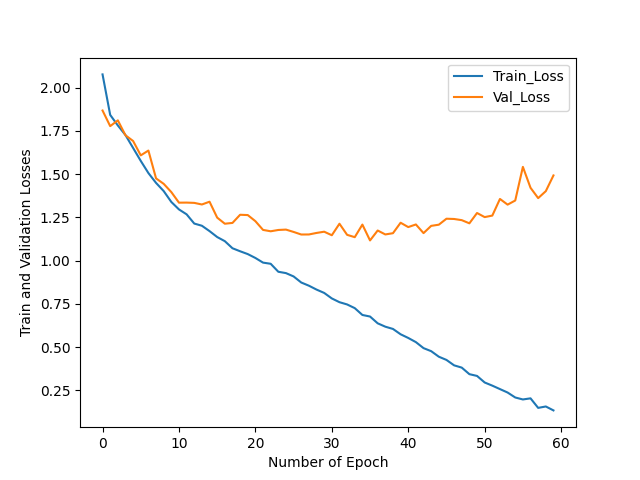
\includegraphics[width=\linewidth]{Figure_1.png}
    \caption{My Trainin and Validation Loss for Best model}
    \label{fig:my_model}
\end{figure}

Figure 2 is from lecture notes. Emprical Error is Trainin loss and true error is the validation error. My saved model is in good models part according to Figure 1 and 2. As I mention above, after 36-40th epoch, validation loss increase which means overfitting. Figure 2 show and support this clearly. 

\begin{figure}[H]
    \centering
    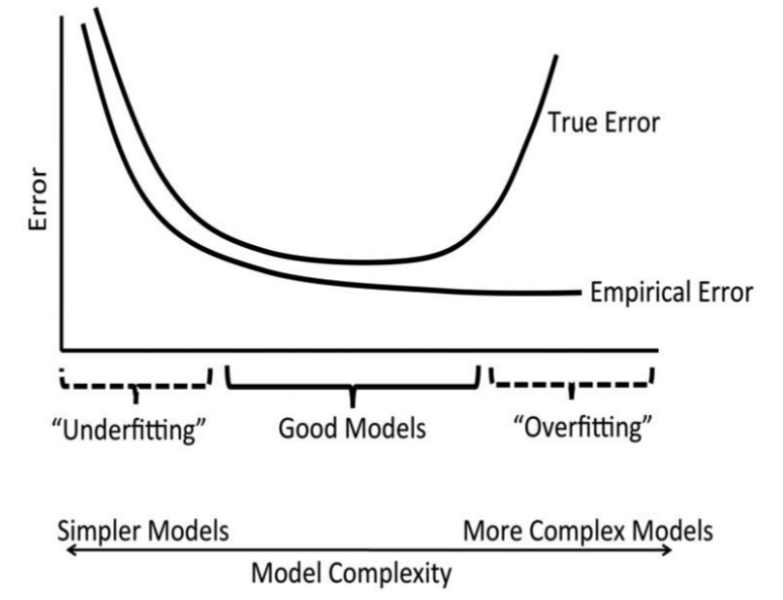
\includegraphics[width=\linewidth]{Lecture_notes_training_and_validation_curve.png}
    \caption{My Trainin and Validation Loss from Lecture Notes}
    \label{fig:lecture_notes}
\end{figure}



\subsection{Overfitting countermeasures}

In order to avoid overfitting, I save the model which have minimum validation loss. My code keep the model and print its loss and accuracy if it is lower than previous minimum validation loss. This enables me to save model which have minimum validation loss for all training.


\section{Comments}

Models which diverge can gave approximately same accuracy result, this show me the power of divergence. When model diverge, its result is equal to random result(0.1). It was nice to see this clearly in the experiments. I also clearly see the overfitting. \\ \\

Number of Layers \\
Before my experiments, I expected when I increase the layer, I can obtain higher accuracy. My experiments supports my expectation. However, if number of hidden layer increase more, it can overfit. Number of layers should be chosen carefully according to problem complexity otherwise, it overfits.  \\ \\

Learning Rate\\

When learning rate is not small enough, model diverge. I obtain best accuracy and minimum loss with learning rate = 0.0003 and 0.0001. They was minimum learning rates I tried. However, if learning rate is too small, it cause the process to get stuck. \\

Number of Neurons \\ 
Increasing number of neurons leads to increase number of feature obtained in the hidden layers. With increase in layers and neurons model complexity increase. This can make model more adaptive but if model is too complex for our problem, it can cause overfitting.\\

Activation Functions \\
Relu, Tanh and Sigmoid all are non linear activation functions. Sigmoid activation function and Tanh activation function use more difficult formulas and are computationally more expensive. Relu is less computationally expensive.\\   

I wanted to add my all loss and accuracy list for all my saved experiment and saved model. Every 6 loss acc values belong to learning rates (0.01, 0.03, 0.001, 0.003, 0.0001, 0.0003) respectively. Other hyperparameters are writen at the top of each 6 model. a result that attracts my attention is loss of model 2 (6.2956). It is due to the fact that it is a single layer and the learning rate is not small enough (0.03)\\ \\

1 layer\\
loss: 2.4197371006011963 and acc: 32.31999969482422	for model number: 1 \\ 
loss: 6.295633316040039 and acc: 21.15999984741211 for model number: 2 \\
loss: 1.699100375175476 and acc: 38.29999923706055 for model number: 3 \\
loss: 1.8511260747909546 and acc: 35.0 for model number: 4 \\
loss: 1.7342185974121094 and acc: 38.959999084472656 for model number: 5 \\
loss: 1.6896936893463135 and acc: 38.619998931884766 for model number: 6 \\
2 layer, Relu, 256 \\
loss: 2.302391529083252 and acc: 10.119999885559082 for model number: 7 \\
loss: 2.3018105030059814 and acc: 11.019999504089355 for model number: 8 \\
loss: 1.251235842704773 and acc: 51.55999755859375 for model number: 9 \\
loss: 1.9628448486328125 and acc: 21.5 for model number: 10 \\
loss: 1.5026451349258423 and acc: 44.79999923706055 for model number: 11 \\
loss: 1.2275702953338623 and acc: 53.79999923706055 for model number: 12 \\
2 layer, Relu, 512 \\
loss: 2.3025012016296387 and acc: 10.119999885559082 for model number: 13 \\
loss: 2.3023319244384766 and acc: 11.019999504089355 for model number: 14 \\
loss: 1.195919156074524 and acc: 52.81999969482422 for model number: 15 \\
loss: 1.971678614616394 and acc: 21.279998779296875 for model number: 16 \\
loss: 1.245701551437378 and acc: 53.21999740600586 for model number: 17 \\
loss: 1.2143890857696533 and acc: 53.84000015258789 for model number: 18 \\
2 layer, Relu, 1024 \\
loss: 2.302229166030884 and acc: 10.119999885559082 for model number: 19 \\
loss: 2.3028337955474854 and acc: 11.019999504089355 for model number: 20 \\
loss: 1.1618438959121704 and acc: 55.65999984741211 for model number: 21 \\
loss: 2.302400827407837 and acc: 10.239999771118164 for model number: 22 \\
loss: 1.2449947595596313 and acc: 52.91999816894531 for model number: 23 \\
loss: 1.1502891778945923 and acc: 56.65999984741211 for model number: 24 \\
2 layer, tanh, 256 \\
loss: 2.3417482376098633 and acc: 9.960000038146973 for model number: 25 \\
loss: 2.35259747505188 and acc: 11.019999504089355 for model number: 26 \\
loss: 1.9856635332107544 and acc: 19.260000228881836 for model number: 27 \\
loss: 2.3149380683898926 and acc: 9.920000076293945 for model number: 28 \\
loss: 1.2745119333267212 and acc: 50.68000030517578 for model number: 29 \\
loss: 1.1772398948669434 and acc: 55.05999755859375 for model number: 30 \\
2 layer, tanh, 512 \\
loss: 2.4207756519317627 and acc: 10.25999927520752 for model number: 31 \\
loss: 2.6945033073425293 and acc: 9.719999313354492 for model number: 32 \\
loss: 1.7400530576705933 and acc: 31.03999900817871 for model number: 33 \\
loss: 2.3245203495025635 and acc: 9.4399995803833 for model number: 34 \\
loss: 1.2350369691848755 and acc: 52.53999710083008 for model number: 35 \\
loss: 1.1589274406433105 and acc: 55.279998779296875 for model number: 36 \\
2 layer, tanh, 1024 \\
loss: 2.4429595470428467 and acc: 10.119999885559082 for model number: 37 \\
loss: 6.429795265197754 and acc: 9.639999389648438 for model number: 38 \\
loss: 2.315912961959839 and acc: 9.920000076293945 for model number: 39 \\
loss: 2.355713129043579 and acc: 10.25999927520752 for model number: 40 \\
loss: 1.231441617012024 and acc: 52.57999801635742 for model number: 41 \\
loss: 1.144446849822998 and acc: 56.19999694824219 for model number: 42 \\
2 layer, sigmoid, 256 \\
loss: 2.325988531112671 and acc: 11.019999504089355 for model number: 43 \\
loss: 2.355567216873169 and acc: 9.639999389648438 for model number: 44 \\
loss: 1.3173824548721313 and acc: 47.81999969482422 for model number: 45 \\
loss: 2.305015802383423 and acc: 10.239999771118164 for model number: 46 \\
loss: 1.5113929510116577 and acc: 44.619998931884766 for model number: 47 \\
loss: 1.1849310398101807 and acc: 55.0 for model number: 48 \\
2 layer, sigmoid, 512 \\
loss: 2.326183795928955 and acc: 9.719999313354492 for model number: 49 \\
loss: 2.3891546726226807 and acc: 9.4399995803833 for model number: 50 \\
loss: 1.3171212673187256 and acc: 48.53999710083008 for model number: 51 \\
loss: 2.314387083053589 and acc: 11.019999504089355 for model number: 52 \\
loss: 1.4625961780548096 and acc: 46.29999923706055 for model number: 53 \\
loss: 1.1680902242660522 and acc: 55.459999084472656 for model number: 54 \\
2 layer, sigmoid, 1024 \\
loss: 2.393315553665161 and acc: 9.920000076293945 for model number: 55 \\
loss: 2.4715189933776855 and acc: 9.639999389648438 for model number: 56 \\
loss: 1.2766320705413818 and acc: 49.03999710083008 for model number: 57 \\
loss: 2.32837176322937 and acc: 9.920000076293945 for model number: 58 \\
loss: 1.3831573724746704 and acc: 47.63999938964844 for model number: 59 \\
loss: 1.1774393320083618 and acc: 55.37999725341797 for model number: 60 \\
3 layer, relu, 256 \\
loss: 1.963399052619934 and acc: 20.799999237060547 for model number: 61 \\
loss: 2.3024065494537354 and acc: 10.25999927520752 for model number: 62 \\
loss: 1.1059772968292236 and acc: 57.79999923706055 for model number: 63 \\
loss: 2.302500009536743 and acc: 10.119999885559082 for model number: 64 \\
loss: 1.1404484510421753 and acc: 56.21999740600586 for model number: 65 \\
loss: 1.137933373451233 and acc: 56.939998626708984 for model number: 66 \\
3 layer, relu , 512 \\
loss: 2.302241086959839 and acc: 11.019999504089355 for model number: 67 \\
loss: 2.303046226501465 and acc: 10.119999885559082 for model number: 68 \\
loss: 1.1091716289520264 and acc: 58.3599967956543 for model number: 69 \\
loss: 1.5253387689590454 and acc: 40.5 for model number: 70 \\
loss: 1.1232572793960571 and acc: 56.91999816894531 for model number: 71 \\
loss: 1.1228394508361816 and acc: 57.53999710083008 for model number: 72 \\
3 layer, relu , 1024 \\
loss: 1.773281455039978 and acc: 30.03999900817871 for model number: 73 \\
loss: 2.302766799926758 and acc: 9.679999351501465 for model number: 74 \\
loss: 1.0888924598693848 and acc: 57.619998931884766 for model number: 75 \\
loss: 1.7348576784133911 and acc: 32.18000030517578 for model number: 76 \\
loss: 1.1335746049880981 and acc: 56.69999694824219 for model number: 77 \\
loss: 1.1126072406768799 and acc: 57.939998626708984 for model number: 78 \\
3 layer, tanh, 256 \\
loss: 2.3428261280059814 and acc: 10.25999927520752 for model number: 79 \\
loss: 2.4260241985321045 and acc: 10.25999927520752 for model number: 80 \\
loss: 2.308587074279785 and acc: 9.639999389648438 for model number: 81 \\
loss: 2.3183255195617676 and acc: 9.639999389648438 for model number: 82 \\
loss: 1.1275438070297241 and acc: 57.05999755859375 for model number: 83 \\
loss: 1.1305831670761108 and acc: 55.57999801635742 for model number: 84 \\
3 layer, tanh, 512 \\
loss: 2.3632678985595703 and acc: 9.639999389648438 for model number: 85 \\
loss: 2.6656577587127686 and acc: 9.679999351501465 for model number: 86 \\
loss: 2.319383144378662 and acc: 9.679999351501465 for model number: 87 \\
loss: 2.3444151878356934 and acc: 9.639999389648438 for model number: 88 \\
loss: 1.0955498218536377 and acc: 58.459999084472656 for model number: 89 \\
loss: 1.1917792558670044 and acc: 54.5 for model number: 90 \\
3 layer, tanh, 1024 \\
loss: 2.4946327209472656 and acc: 10.239999771118164 for model number: 91 \\
loss: 4.41921329498291 and acc: 10.239999771118164 for model number: 92 \\
loss: 2.3225767612457275 and acc: 9.719999313354492 for model number: 93 \\
loss: 2.352379083633423 and acc: 9.960000038146973 for model number: 94 \\
loss: 1.1109501123428345 and acc: 57.279998779296875 for model number: 95 \\
loss: 1.153237223625183 and acc: 54.57999801635742 for model number: 96 \\
3 layer, sigmoid, 256 \\
loss: 2.3166260719299316 and acc: 9.719999313354492 for model number: 97 \\
loss: 2.3603124618530273 and acc: 10.239999771118164 for model number: 98 \\
loss: 1.337018609046936 and acc: 48.07999801635742 for model number: 99 \\
loss: 2.307936668395996 and acc: 10.25999927520752 for model number: 100 \\
loss: 1.1767425537109375 and acc: 54.29999923706055 for model number: 101 \\
loss: 1.1583646535873413 and acc: 55.279998779296875 for model number: 102 \\
3 layer, sigmoid, 512 \\
loss: 2.33615779876709 and acc: 10.119999885559082 for model number: 103 \\
loss: 2.4607183933258057 and acc: 11.019999504089355 for model number: 104 \\
loss: 1.5157721042633057 and acc: 38.18000030517578 for model number: 105 \\
loss: 2.311610460281372 and acc: 10.25999927520752 for model number: 106 \\
loss: 1.1662434339523315 and acc: 54.69999694824219 for model number: 107 \\
loss: 1.158468246459961 and acc: 55.02000045776367 for model number: 108 \\
3 layer, sigmoid, 1024 \\
loss: 2.384624481201172 and acc: 11.019999504089355 for model number: 109 \\
loss: 2.6658804416656494 and acc: 10.119999885559082 for model number: 110 \\
loss: 1.8033078908920288 and acc: 30.079999923706055 for model number: 111 \\
loss: 2.309619188308716 and acc: 10.239999771118164 for model number: 112 \\
loss: 1.1667876243591309 and acc: 54.939998626708984 for model number: 113 \\
loss: 1.196830153465271 and acc: 53.68000030517578 for model number: 114 \\


\end{document}

